\documentclass{article}

\usepackage{fancyhdr, lastpage}
\usepackage[inline]{enumitem}
\usepackage{listings}
\usepackage[scaled=0.95]{inconsolata}  % Use a monospaced font, like Inconsolata
\usepackage{wasysym}
\usepackage{booktabs}
\usepackage{multicol}
\usepackage{siunitx}
\usepackage{xfrac}
\usepackage{extramarks}
\usepackage{amsmath, amsthm, amsfonts, mathtools, empheq}
\usepackage{caption}
\usepackage{xcolor}
\usepackage{tikz}
\usepackage[most]{tcolorbox}
\usepackage{pagecolor} %% for dark background

\usetikzlibrary{tikzmark, calc}

\pagecolor{black}
\definecolor{magenta}{RGB}{255,0,255}
\definecolor{cyan}{RGB}{0,255,255}
\definecolor{white}{RGB}{255,255,255}
\definecolor{red}{RGB}{255,0,0}
\definecolor{green}{RGB}{0,255,0}
\definecolor{orange}{RGB}{255,165,0}
\definecolor{yellow}{RGB}{255,255,0}
\definecolor{blue}{RGB}{10,10,255}

\newcommand{\cw}{\color{white}}
\newcommand{\cm}{\color{magenta}}
\newcommand{\cc}{\color{cyan}}
\newcommand{\cred}{\color{red}}
\newcommand{\cb}{\color{blue}}
\newcommand{\cg}{\color{green}}
\newcommand{\cy}{\color{yellow}}
\newcommand{\co}{\color{orange}}

% %% make subscripts smaller
% \begingroup\lccode`~=`_
% \lowercase{\endgroup\def~}#1{_{\scriptscriptstyle#1}}
% \AtBeginDocument{\mathcode`_="8000 \catcode`_=12 }

\topmargin=-0.45in
\evensidemargin=0in
\oddsidemargin=0in
\textwidth=6.5in
\textheight=9.0in
\headsep=0.25in

\linespread{1.1}

\pagestyle{fancy}
\lhead{\hmwkAuthorName}
\chead{\hmwkTitle}
\rhead{\hmwkClass}
\lfoot{\lastxmark}
\cfoot{Page \thepage\ of \pageref{LastPage}}

\renewcommand\headrulewidth{0.4pt}
\renewcommand\footrulewidth{0.4pt}

\setlength\parindent{0pt}

%
% Create Problem Sections
%

\newcommand{\enterProblemHeader}[1]{
    \nobreak\extramarks{}{Problem \arabic{#1} continued on next page\ldots}\nobreak{}
    \nobreak\extramarks{Problem \arabic{#1} (continued)}{Problem \arabic{#1} continued on next page\ldots}\nobreak{}
}

\newcommand{\exitProblemHeader}[1]{
    \nobreak\extramarks{Problem \arabic{#1} (continued)}{Problem \arabic{#1} continued on next page\ldots}\nobreak{}
    \stepcounter{#1}
    \nobreak\extramarks{Problem \arabic{#1}}{}\nobreak{}
}

\setcounter{secnumdepth}{0}
\newcounter{partCounter}
\newcounter{homeworkProblemCounter}
\setcounter{homeworkProblemCounter}{1}
\nobreak\extramarks{Problem \arabic{homeworkProblemCounter}}{}\nobreak{}

%
% Homework Problem Environment
%
% This environment takes an optional argument. When given, it will adjust the
% problem counter. This is useful for when the problems given for your
% assignment aren't sequential. See the last 3 problems of this template for an
% example.
%
\newenvironment{homeworkProblem}[1][-1]{
    \ifnum#1>0
        \setcounter{homeworkProblemCounter}{#1}
    \fi
    \section{Problem \arabic{homeworkProblemCounter}}
    \setcounter{partCounter}{1}
    \enterProblemHeader{homeworkProblemCounter}
}{
    \exitProblemHeader{homeworkProblemCounter}
}

%
% Homework Details
%   - Title
%   - Due date
%   - Class
%   - Section/Time
%   - Instructor
%   - Author
%

\newcommand{\hmwkTitle}{Homework\ \#3}
\newcommand{\hmwkDueDate}{April 1, 2024}
\newcommand{\hmwkClass}{EGR 5110}
\newcommand{\hmwkClassTime}{}
\newcommand{\hmwkClassInstructor}{Professor Nissenson}
\newcommand{\hmwkAuthorName}{\textbf{Francisco Sanudo}}

%
% Title Page
%

\title{
    \vspace{2in}
    \textmd{\textbf{\hmwkClass:\ \hmwkTitle}}\\
    \normalsize\vspace{0.1in}\small{Due\ on\ \hmwkDueDate\ at 11:59pm}\\
    \vspace{0.1in}\large{\textit{\hmwkClassInstructor\ \hmwkClassTime}}
    \vspace{3in}
}

\author{\hmwkAuthorName}
\date{}

\renewcommand{\part}[1]{\textbf{\large Part \Alph{partCounter}}\stepcounter{partCounter}\\}

%
% Various Helper Commands
%


% For derivatives
\newcommand{\deriv}[2]{\frac{d#1}{d#2}}

% For partial derivatives
\newcommand{\pderiv}[2]{\frac{\partial}{\partial #1} (#2)}

% Redefine \dfrac if you want all fractions to be in display style automatically
\newcommand{\ddfrac}[2]{\frac{\displaystyle #1}{\displaystyle #2}}

% Alias for the Solution section header
\newcommand{\solution}{\textbf{\large Solution}}

% Define the caption format
\DeclareCaptionFormat{white}{%
  \color{white}#1#2#3\par
}

% Apply the caption format to figures
\captionsetup[figure]{format=white}

%% Box settings
% \setlength{\fboxsep}{9pt} % Adjust the padding thickness here
\setlength{\fboxrule}{1pt} % Adjust the border thickness here

% The \dimexpr\linewidth-2\fboxsep-2\fboxrule\relax calculation ensures that the width of the minipage is reduced by twice the padding and twice the border width, as there is padding and border on both the left and right sides.
\newcommand{\boxsettings}{\dimexpr\linewidth-2\fboxsep-2\fboxrule\relax}

% Set default text color
\cw

\begin{document}

\maketitle

\pagebreak

\section{Background}

The \color{magenta} three-body problem \color{white} is a dynamics problem in which a relatively small object is influenced by two much more massive bodies, and the two massive bodies have circular orbits about their barycenter (combined center of mass). The following nonlinear second-order differential equations describe the motion of a spacecraft in orbit about the Earth and Moon:
\color{cyan}
\begin{align}
    \deriv{^2 x}{t^2} & = 2\deriv{y}{t} + x - \frac{\tilde{\mu} \left(x+\mu\right)}{r_1^3} - \frac{\mu \left(x-\tilde{\mu}\right)}{r_2^3} - f_d \deriv{x}{t}
    \label{eq:ODE1}                                                                                                                                          \\
    \deriv{^2 y}{t^2} & = -2\deriv{x}{t} + y - \frac{\tilde{\mu}y}{r_1^3} - \frac{\mu y}{r_2^3} - f_d\deriv{y}{t}
    \label{eq:ODE2}
\end{align}
\color{white} where
\color{orange}
\begin{equation*}
    \mu = \frac{1}{82.45} \qquad \tilde{\mu} = 1 - \mu \qquad r_1^2 = \left(x+\mu\right)^2 + y^2 \qquad r_2^2 = \left(x-\tilde{\mu}\right)^2 + y^2
\end{equation*}

\color{white}

$\mu$ is the ratio of the Moon's mass to Earth's mass, $r_1$ is the distance from the Earth’s center to the
spacecraft, $r_2$ is the distance from the Moon’s center to the spacecraft, and $f_d$ is a deceleration/acceleration
coefficient.

\vspace{\baselineskip}

The equations are derived from Newton’s law of motion and the inverse square law of gravitation. We are taking the perspective of someone in a reference frame that is rotating at the same angular speed as the Earth and Moon about their barycenter, so the Earth and Moon appear fixed in this reference frame (only the spaceship will appear to move). It is assumed that the three bodies move in a 2D plane and the x-axis forms a line through the Earth and Moon. The origin is located at the barycenter, the Moon’s center of mass is located at point (1-$\mu$,0), and the Earth’s center of mass is located at point (-$\mu$,0).

\vspace{\baselineskip}

The equation uses normalized units for space and time. A normalized spatial unit of 1 in this coordinate
system is equal to the characteristic length of the system, which is the distance between the earth and moon
($d$ = 384,400 km). One normalized time unit is equal to the characteristic time:
\begin{equation*}
    t = \sqrt{\frac{d^3}{G\left(m_{earth} + m_{moon}\right)}}
\end{equation*}
where $G$ = gravitational constant = $6.67 \times 10^{-11} \SI{}{\ \N\cdot\m^2/\kg^2}$, $m_{earth} = 5.972 \times 10^{24}$ kg, and $m_{moon} = 7.348 \times 10^{22}$ kg. This means one normalized time unit is $3.75 \times 10^5$ s, or 4.34 days.

\pagebreak

\section{System of Coupled First-Order ODEs}

The goal of this assignment is to build an RK4 method ODE solver that solves a set of coupled first-order ODEs from an initial time $t_0$ to a final time $t_f$.

\vspace{\baselineskip}

Recall the first order ODE
\begin{equation*}
    \deriv{y}{x} = f(x,y) \quad \text{ with } \quad y(x_0) = y_0
\end{equation*}

Any higher order ODE, that can be solved for the highest derivative term, can be written as a system of first-order ODEs (\color{magenta} One $n^{\textrm{th}}$ order ODE $\rightarrow$ $n$ 1st order ODEs\color{white}). Applying this to Equation~(\ref{eq:ODE1}) and (\ref{eq:ODE2}):

\vspace{\baselineskip}

Let
\begin{align*}
    x_1 & = x       \\
    x_2 & = y       \\
    x_3 & = \dot{x} \\
    x_4 & = \dot{y}
\end{align*}
Thus,
\begin{align*}
    \dot{x}_1 & = \dot{x} = x_3                                                                                                                       & \dot{x}_2                                                                                  & = \dot{y} = x_4
    \\
    \dot{x}_3 & = \ddot{x} = 2\dot{y} + x - \frac{\tilde{\mu} \left(x+\mu\right)}{r_1^3} - \frac{\mu \left(x-\tilde{\mu}\right)}{r_2^3} - f_d \dot{x}
              & \dot{x}_4                                                                                                                             & = \ddot{y} = -2\dot{x} + y - \frac{\tilde{\mu}y}{r_1^3} - \frac{\mu y}{r_2^3} - f_d\dot{y}
    \\
              & = 2x_4 + x_1 - \frac{\tilde{\mu} \left(x_1+\mu\right)}{r_1^3} - \frac{\mu \left(x_1-\tilde{\mu}\right)}{r_2^3} - f_d x_3
              &                                                                                                                                       & = -2x_3 + x_2 - \frac{\tilde{\mu}x_2}{r_1^3} - \frac{\mu x_2}{r_2^3} - f_d x_4
\end{align*}

Let $\bf{X}$ denote the column vector containing the states $x_1,x_2,x_3,x_4$. This means that

\begin{empheq}[box=\fbox]{align*}
    \bf{X}
    &= \begin{bmatrix}
        x_1 \\
        x_2 \\
        x_3 \\
        x_4
    \end{bmatrix},
    \qquad \color{cyan} \dot{\bf{X}} =
    \begin{bmatrix}
        \dot{x}_1 \\
        \dot{x}_2 \\
        \dot{x}_3 \\
        \dot{x}_4
    \end{bmatrix}
    =
    \begin{bmatrix}
        x_3                                                                                                                        \\[0.2cm]
        x_4                                                                                                                        \\[0.2cm]
        2x_4 + x_1 - \ddfrac{\tilde{\mu} \left(x_1+\mu\right)}{r_1^3} - \ddfrac{\mu \left(x_1-\tilde{\mu}\right)}{r_2^3} - f_d x_3 \\[0.2cm]
        -2x_3 + x_2 - \ddfrac{\tilde{\mu} \, x_2}{r_1^3} - \ddfrac{\mu \, x_2}{r_2^3} - f_d x_4
    \end{bmatrix}
\end{empheq}

\vspace{\baselineskip}

This is a system of coupled first-order ordinary differential equations that require a total of 4 initial condtions to solve. The benefit of writing the equations in this form is that \color{magenta} two 2nd-order equations are reduced to four 1st-order equations \color{white} that can be simultaneously solved for the spacecraft's states (position and velocity), and hence provide us with the time histories of the spacecraft's trajectory relative to the Earth and Moon in the rotating coordinate system.

\vspace{\baselineskip}

The system $\dot{\bf{X}} = f(t,\bf{X})$ can now be solved using the RK4 algorithm for the position and velocity of the spacecraft at $N$ discrete times from $t_0$ to $t_f$, when provided the vector comprising the components of the states at time $t_0$:

\begin{equation*}
    \textbf{X}(0) =
    \begin{bmatrix}
        x_1 & x_2 & x_3 & x_4
    \end{bmatrix}^T(0)
    =
    \begin{bmatrix}
        x_0 & y_0 & \dot{x}_0 & \dot{y}_0
    \end{bmatrix}^T
\end{equation*}

\pagebreak

\section{Simulations}
It is possible that the number of steps input by the user ($N$) is too small to get accurate results in the RK4 alogrithm. So how do we determine the number of steps required to obtain an accurate solution?

\vspace{\baselineskip}

One crude approach is to look at the global error. This means doubling the number of steps (cut the step size in half) until the relative difference in the final position falls below a tolerance tol. The termination criterion is:
\begin{equation*}
    \left|\frac{y_2(x_f) - y_1(x_f)}{y_2(x_f)}\right| < \textrm{tol}
\end{equation*}
where $y_1(x_f)$ is the solution at the final step for a certain $\Delta x$, and $y_2(x_f)$ is the solution at the final step for $\Delta x/2$.

\vspace{\baselineskip}

I will explore two scenarios. For both scenarios, I will create two plots (described below) and include a table of $N$, $\textrm{d}t$, $r_1$, and the test criterion below:
\color{cyan}
\begin{equation*}
    \left|\frac{r_1(\textrm{end})_{2N} - r_1(\textrm{end})_N}{r_1(\textrm{end})_{2N}}\right|
\end{equation*}
\color{white}
where $r_1(\textrm{end})_N$ is the radial distance from the earth’s center to the spaceship at the end of the simulation using a certain step size, and $r_1(\textrm{end})_{2N}$ is the radial distance from the earth’s center to the spaceship at the end of the simulation using the smaller step size (one-half the step size used to calculate $r_1(\textrm{end})_N$).

\vspace{\baselineskip}

We shall start with $N$ = 1000 and use a tolerance of tol = 0.01.

\pagebreak

\subsection{Scenario 1}

Initial Conditions:
\begin{multicols}{4}
    \begin{itemize}
        \item $x(0)$ = 1.2
        \item $y(0)$ = 0
        \item $v_x(0)$ = 0
        \item $f_d$ = 0
        \item $v_y(0)$ = -1.0493571
    \end{itemize}
\end{multicols}

\textbf{Note}: All quantities are in normalized units.

\vspace{\baselineskip}

These initial conditions correspond to a spacecraft initially on the far side of the moon. The trajectory will be calculated from $t$ = 0 to 15 normalized time units.

\vspace{\baselineskip}

The results are shown below:

\begin{figure}[h]
    \centering
    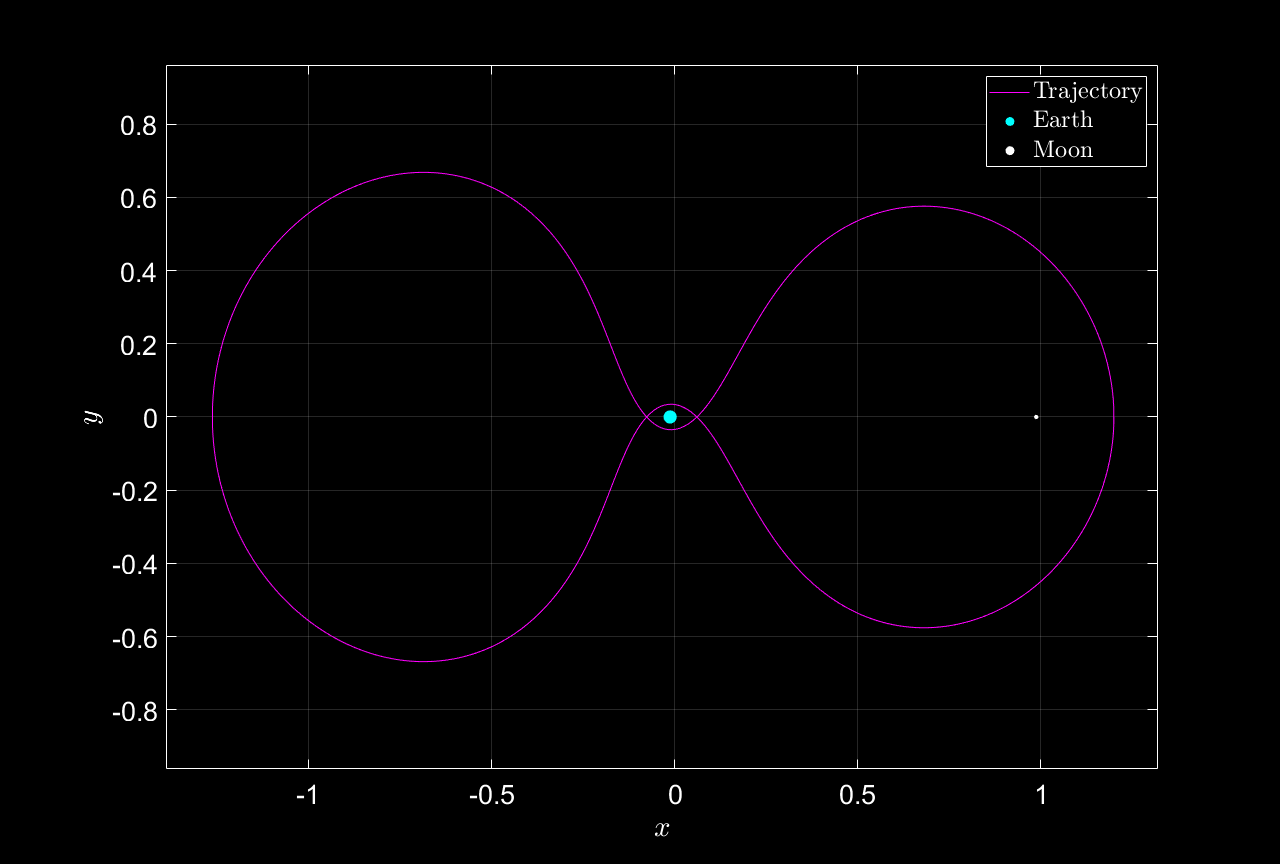
\includegraphics[width=\textwidth]{fig/trajectory1.png}
    \caption{Spacecraft Trajectory about the Earth \& Moon in the Synodic Frame}
    \label{fig1}
\end{figure}

\pagebreak

\begin{figure}[!h]
    \centering
    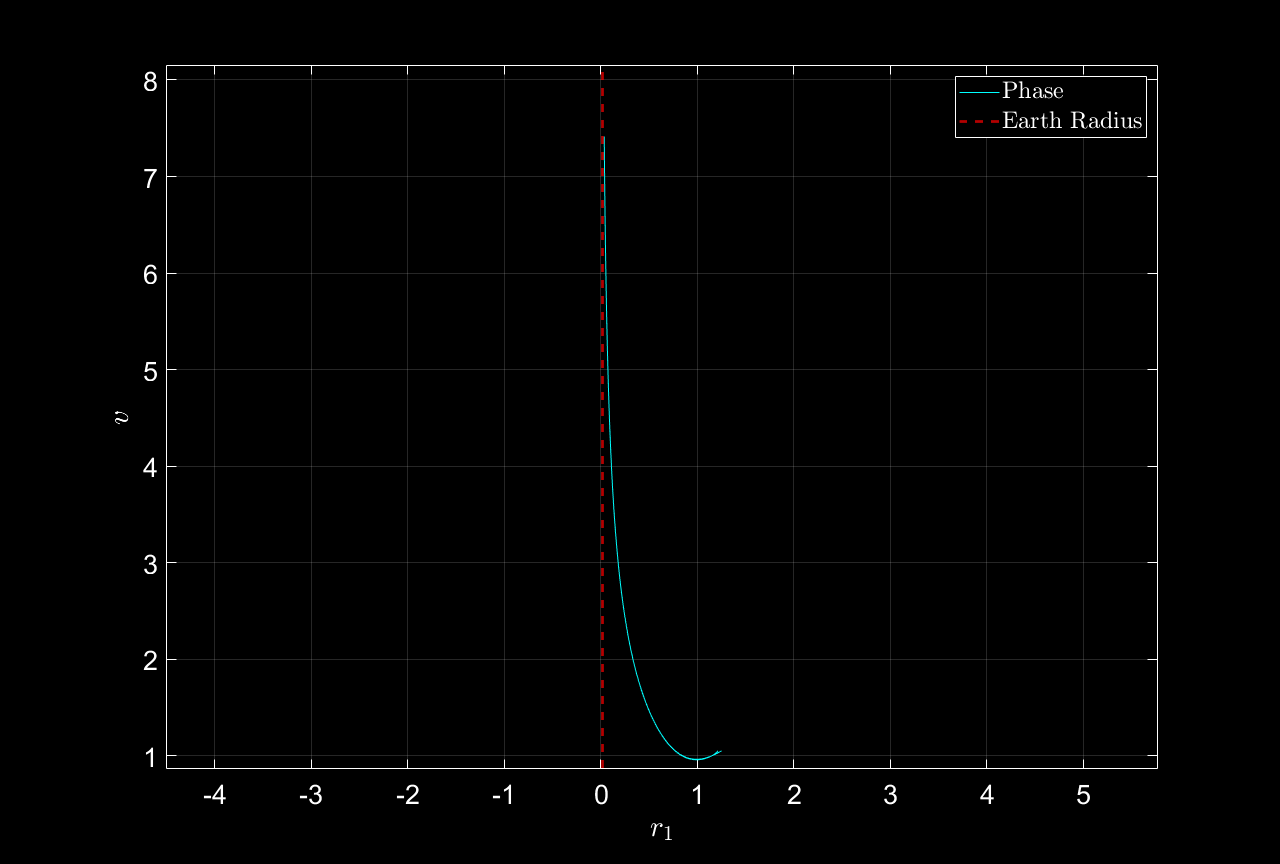
\includegraphics[width=\textwidth]{fig/phase1.png}
    \caption{Phase Space, \textit{Speed vs. Radial Distance from Earth}}
    \label{fig2}
\end{figure}


\begin{table}[h]
    \centering
    \caption{\cw Effects of Increasing the Number of Steps for Scenario 1}
    \begin{tabular}{cccc} \toprule
        {$N$} & {$\mathrm{d}t$}    & {$r_1$}  & {$\mathrm{Test \ Criterion}$}                 \\ \midrule
        1000  & 0.0150             & 14.7302  & N/A                                           \\
        2000  & 0.0075             & 212.1128 & 0.9306                                        \\
        4000  & 0.0038             & 7.0135   & 29.2437                                       \\
        8000  & 0.0019             & 1.2056   & 4.8173                                        \\
        16000 & $\SI{9.3750E-4}{}$ & 1.1816   & 0.0203                                        \\
        32000 & $\SI{4.6875e-4}{}$ & 1.1808   & \color{magenta}$\SI{6.3125e-4}{}$ \cw $<$ tol \\ \bottomrule
    \end{tabular}
    \label{tab:table1}
\end{table}

Upon completion of the simulation, the closest proximity to the Earth's surface was determined to be $r_1$ = 6947.40 km.

\pagebreak

\subsection{Scenario 2}

Initial Conditions:
\begin{multicols}{4}
    \begin{itemize}
        \item $x(0)$ = 1.2
        \item $y(0)$ = 0
        \item $v_x(0)$ = 0
        \item $f_d$ = 1
        \item $v_y(0)$ = -1.0493571
    \end{itemize}
\end{multicols}

\textbf{Note}: All quantities are in normalized units.

\vspace{\baselineskip}

These initial conditions are identical to the ones from the Scenario 1, but we set $f_d$ = 1, which corresponds to rockets firing in the retrograde direction with constant thrust through the entire flight. The trajectory will be calculated from $t$ = 0 to 4 normalized time units.

\vspace{\baselineskip}

The results are shown below:

\begin{figure}[h]
    \centering
    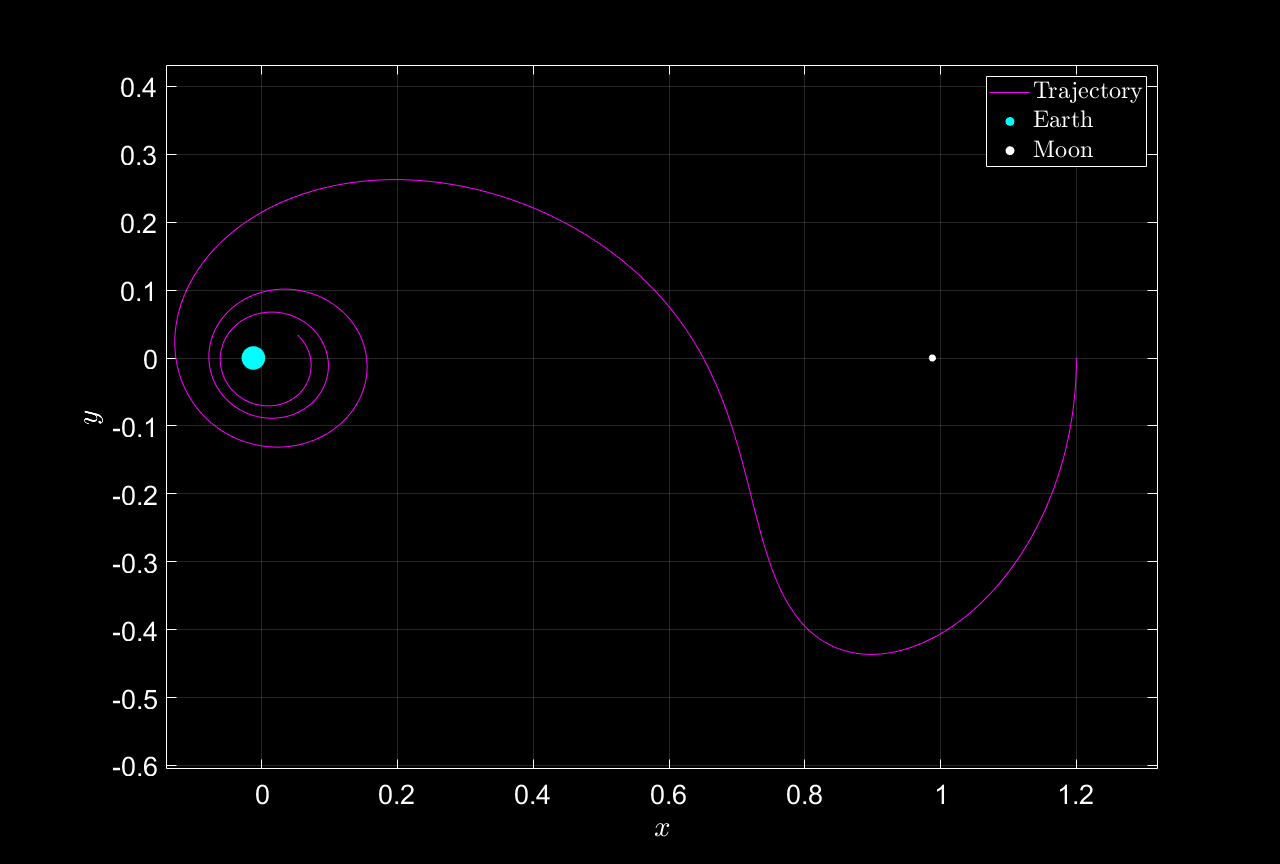
\includegraphics[width=\textwidth]{fig/trajectory2.png}
    \caption{Spacecraft Trajectory about the Earth \& Moon in the Synodic Frame}
    \label{fig3}
\end{figure}

\pagebreak

\begin{figure}[!h]
    \centering
    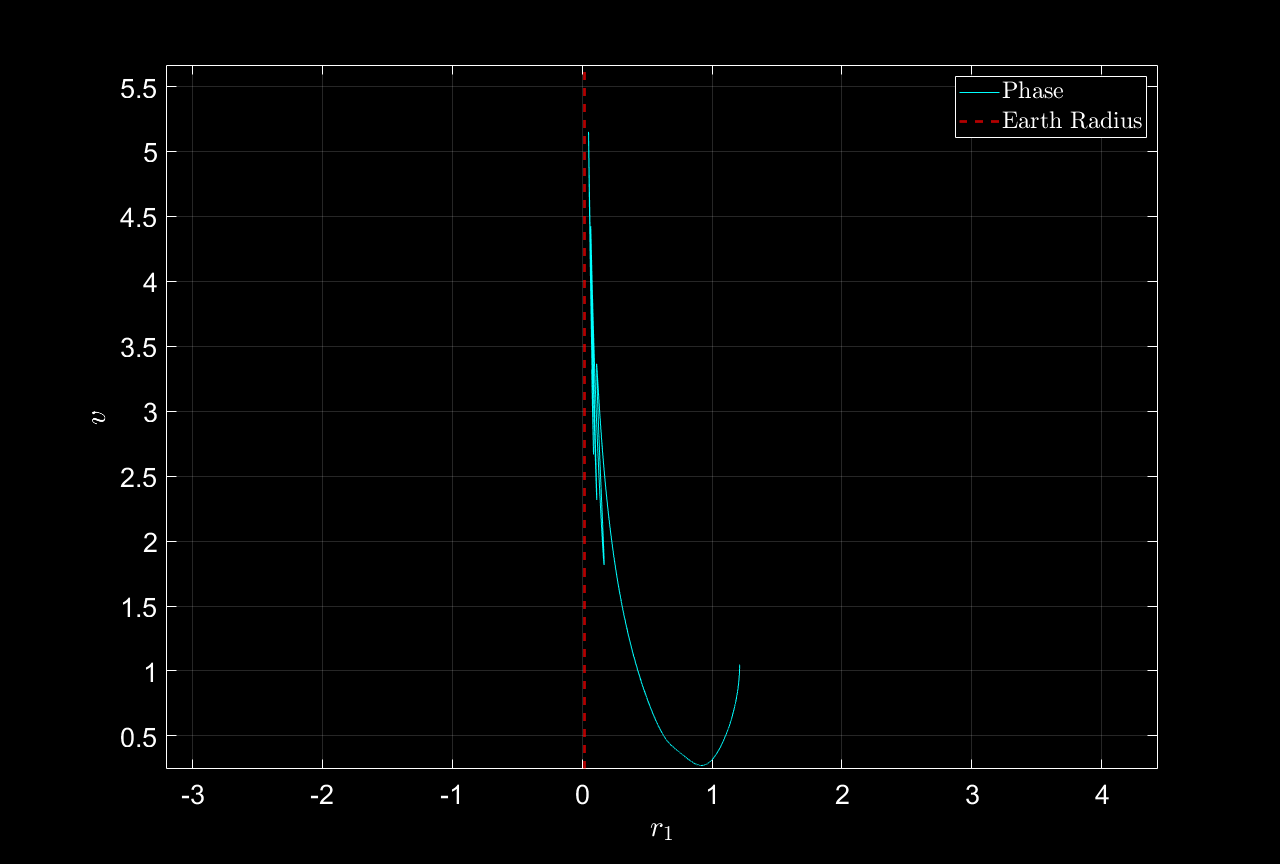
\includegraphics[width=\textwidth]{fig/phase2.png}
    \caption{Phase Space, \textit{Speed vs. Radial Distance from Earth}}
    \label{fig4}
\end{figure}


\begin{table}[h]
    \centering
    \caption{\cw Effects of Increasing the Number of Steps for Scenario 2}
    \begin{tabular}{cccc} \toprule
        {$N$} & {$\mathrm{d}t$} & {$r_1$} & {$\mathrm{Test \ Criterion}$}      \\ \midrule
        1000  & 0.0040          & 0.0767  & N/A                                \\
        2000  & 0.0020          & 0.0748  & 0.0249                             \\
        4000  & 0.0010          & 0.0738  & 0.0144                             \\
        8000  & 0.0005          & 0.0732  & \color{magenta} 0.0075 \cw $<$ tol \\ \bottomrule
    \end{tabular}
    \label{tab:table2}
\end{table}

Extending the simulation duration would lead to the solution diverging towards infinity. This outcome is anticipated, as the spacecraft gradually spirals in towards Earth under a sustained deceleration, causing the radial distance $r_1$ to approach zero. A close examination of the equations of motion, as shown in \eqref{eq:ODEset}, reveals that as $r_1$ diminishes towards zero, both $\dot{v}_x$ and $\dot{v}_y$ tend towards negative infinity. To keep things in check, it's a good idea to add a quick check in the numerical code, making sure $r_1$ doesn't dip below Earth's radius. This would stop the simulation from spiraling out of control (my code doesn't do this, yet).

\pagebreak

\section{Lagrange Points}

Lagrange points are special locations in the CR3BP rotating reference frame where if one were to place an object with negligible mass at a Lagrange point, with zero velocity, it will remain stationary with respect to the rotating frame.

\vspace{\baselineskip}

In vector equation terms, we can define Lagrange points as locations where:
\begin{equation*}
    \vec{r}(t) = \vec{r}(0) \rightarrow \deriv{\vec{r}}{t} = \vec{0} \rightarrow \deriv{^2\vec{r}}{t^2} = \vec{0}
\end{equation*}
i.e., the position vector is constant for all time and equal to it's initial position. Therefore, the first and second deivatives of the position vector must be zero at all times.

\vspace{\baselineskip}

Recall our state vector and the derivative of our states:

\begin{equation*}
    \bf{X}
    = \begin{bmatrix}
        \vec{r} \\
        \vec{v}
    \end{bmatrix}
    = \begin{bmatrix}
        x   \\
        y   \\
        v_x \\
        v_y
    \end{bmatrix},
    \qquad \dot{\bf{X}} =
    \begin{bmatrix}
        v_x                                                                                                                  \\[0.2cm]
        v_y                                                                                                                  \\[0.2cm]
        2v_y + x - \ddfrac{\tilde{\mu} \left(x+\mu\right)}{r_1^3} - \ddfrac{\mu \left(x-\tilde{\mu}\right)}{r_2^3} - f_d v_x \\[0.2cm]
        -2v_x + y - \ddfrac{\tilde{\mu}y}{r_1^3} - \ddfrac{\mu y}{r_2^3} - f_d v_y
    \end{bmatrix}
\end{equation*}

If $\displaystyle \deriv{\vec{r}}{t} = \vec{v} = \vec{0}$ and $\displaystyle \deriv{^2\vec{r}}{t^2} = \deriv{\vec{v}}{t} = \vec{0}$, then the derivative of our state vector $\dot{\textbf{X}}$ must be zero:

\begin{equation*}
    \dot{\bf{X}} =
    \begin{bmatrix}
        v_x                                                                                                                  \\[0.2cm]
        v_y                                                                                                                  \\[0.2cm]
        2v_y + x - \ddfrac{\tilde{\mu} \left(x+\mu\right)}{r_1^3} - \ddfrac{\mu \left(x-\tilde{\mu}\right)}{r_2^3} - f_d v_x \\[0.2cm]
        -2v_x + y - \ddfrac{\tilde{\mu}y}{r_1^3} - \ddfrac{\mu y}{r_2^3} - f_d v_y
    \end{bmatrix}
    =
    {
    \renewcommand{\arraystretch}{1.2} % Adjusts the row spacing 
    \begin{bmatrix}
        0 \\
        0 \\
        0 \\
        0
    \end{bmatrix}
    }
\end{equation*}

Since we asserted that $\displaystyle \deriv{\vec{v}}{t} = \left[v_x \ v_y\right]^T = \vec{0}$, then we must find the values of $x$ and $y$ such that:

\begin{equation}
    \begin{bmatrix}
        \textcolor{magenta}{x} - \ddfrac{\tilde{\mu} \left(\textcolor{magenta}{x}+\mu\right)}{r_1^3} - \ddfrac{\mu \left(\textcolor{magenta}{x}-\tilde{\mu}\right)}{r_2^3} \\[0.2cm]
        \textcolor{magenta}{y} - \ddfrac{\tilde{\mu}\textcolor{magenta}{y}}{r_1^3} - \ddfrac{\mu \textcolor{magenta}{y}}{r_2^3}
    \end{bmatrix}
    =
    {
    \renewcommand{\arraystretch}{1.2} % Adjusts the row spacing 
    \begin{bmatrix}
        0 \\
        0
    \end{bmatrix}
    }
    \label{eq:roots}
\end{equation}

From Equation~(\refeq{eq:roots}), we have

\begin{equation}
    \textcolor{magenta}{y} \left( 1 - \ddfrac{\left(1-\cred\mu\cw\right)}{\cc r_1 \cw ^3} - \ddfrac{\cred\mu\cw}{\cg r_2 \cw ^3} \right) = 0
    \label{eq:rootsY}
\end{equation}

while the individual terms $\mu$, $1-\mu$, $r_1^3$, and $r_2^3$ cannot be zero based on the given constraints, the value of the entire expression within the parentheses could potentially be zero if the terms subtract to zero. However, let's look at the case where $y$ = 0 -- corresponding to solutions that are collinear with the x-axis -- and later revisit the case where $y \neq 0$.

\pagebreak

\subsection{Collinear Solutions \texorpdfstring{($y = 0$)}{}}

From Equation~(\refeq{eq:roots}), we have
\begin{equation}
    \cm x \cw - \ddfrac{\left(1 - \cred \mu \cw \right) \left(\cm x \cw + \cred \mu \cw\right)}{\cc r_1 \cw ^3} - \ddfrac{\cred \mu \cw \left(\cm x \cw - 1 + \cred\mu\cw\right)}{\cg r_2 \cw ^3} = 0
    \label{eq:rootsX}
\end{equation}

Recall that
\begin{equation*}
    \cc r_1 \cw ^2 = \left(\cm x \cw + \cred\mu\cw\right)^2 + \cm y \cw ^2 \qquad \cg r_2 \cw ^2 = \left(\cm x \cw - 1 + \cred\mu\cw\right)^2 + \cm y \cw ^2
\end{equation*}

By setting $y = 0$, Equation~\eqref{eq:rootsX} becomes
\begin{equation}
    \cm x \cw \, \tikzmarknode{A}{-} \, \ddfrac{\left(1 - \cred \mu \cw \right) \left(\cm x \cw + \cred \mu \cw\right)}{\left(\sqrt{\left(\cm x \cw + \cred\mu\cw\right)^2}\right)^3} \, \tikzmarknode{B}{-} \, \ddfrac{\cred \mu \cw \left(\cm x \cw - 1 + \cred\mu\cw\right)}{\left(\sqrt{\left(\cm x \cw - 1 + \cred\mu\cw\right)^2}\right)^3} = 0  \\
    \label{eq:eq6}
    \begin{tikzpicture}[overlay, remember picture]
        % Calculate points for the start and end of the blue arrow
        \coordinate (startBlue) at ($(A)+(-0.2, -0.9)$);
        \coordinate (endBlue) at ($(startBlue)+(0.2, 0.75)$);

        % Calculate points for the start and end of the green arrow
        \coordinate (startGreen) at ($(B)+(-0.2, -0.9)$);
        \coordinate (endGreen) at ($(startGreen)+(0.2, 0.75)$);

        % Draw the blue arrow
        \draw[blue,-latex, thick] (startBlue) -- (endBlue);

        % Draw the green arrow
        \draw[green,-latex, thick] (startGreen) -- (endGreen);
    \end{tikzpicture}
\end{equation}

In Equation~\eqref{eq:eq6}, there may be a temptation to cancel terms prematurely but this could potentially eliminate valid solutions. Let's consider four scenarios that correspond to the second and third terms in \eqref{eq:eq6} being either positive or negative before further simplifying the equation.

\vspace{\baselineskip}

\underline{Scenario 1}: \quad $\cm x \cw + \cred \mu \cw > 0$, \quad $\cm x \cw - 1 + \cred \mu \cw < 0$ \quad $\longrightarrow$ \quad $\cm x \cw > - \cred \mu \cw$, \quad $\cm x \cw < 1 - \cred \mu \cw$

\begin{center}
    \vspace{7pt}
    \begin{tikzpicture}
        % Draw the horizontal line
        \draw[thick] (-3,0) -- (4,0);

        % Draw the ticks and labels
        \draw[thick] (-2,0.2) -- (-2,-0.2) node[below] {$- \cred \mu$};
        \draw[thick] (-1.2,0.2) -- (-1.2,-0.2) node[below] {0};
        \draw[thick] (3,0.2) -- (3,-0.2) node[below] {$1-\cred \mu$};

        % Draw the blue arrow with square
        \filldraw[blue] (-1.95,0.65) rectangle (-2.05,0.75); % Make square thinner
        \draw[blue, very thick, -latex] (-2,0.7) -- (4,0.7); % Start slightly above the line

        % Draw the green arrow with square
        \filldraw[green] (2.95,0.35) rectangle (3.05,0.45); % Make square thinner
        \draw[green, very thick, -latex] (3,0.4) -- (-3,0.4); % Start slightly above the line
        % Add a node for text at a certain position
        \node[anchor=west] at (-5,0) {$\cb >$,$\cg <$};
    \end{tikzpicture}
\end{center}

This corresponds to a solution that lies between the two bodies.

\vspace{\baselineskip}

\underline{Scenario 2}: \quad $\cm x \cw + \cred \mu \cw > 0$, \quad $\cm x \cw - 1 + \cred \mu \cw > 0$ \quad $\longrightarrow$ \quad $\cm x \cw > - \cred \mu \cw$, \quad $\cm x \cw > 1 - \cred \mu \cw$

\begin{center}
    \vspace{7pt}
    \begin{tikzpicture}
        % Draw the horizontal line
        \draw[thick] (-3,0) -- (4,0);

        % Draw the ticks and labels
        \draw[thick] (-2,0.2) -- (-2,-0.2) node[below] {$- \cred \mu$};
        \draw[thick] (-1.2,0.2) -- (-1.2,-0.2) node[below] {0};
        \draw[thick] (3,0.2) -- (3,-0.2) node[below] {$1-\cred \mu$};

        % Draw the blue arrow with square
        \filldraw[blue] (-1.95,0.65) rectangle (-2.05,0.75); % Make square thinner
        \draw[blue, very thick, -latex] (-2,0.7) -- (4,0.7); % Start slightly above the line

        % Draw the green arrow with square
        \filldraw[green] (2.95,0.35) rectangle (3.05,0.45); % Make square thinner
        \draw[green, very thick, -latex] (3,0.4) -- (4,0.4); % Start slightly above the line
        % Add a node for text at a certain position
        \node[anchor=west] at (-5,0) {$\cb >$, $\cg >$};
    \end{tikzpicture}
\end{center}

From above, we can see that both inequalities are true when $\cm x \cw > 1 - \cred \mu \cw$. We don't know what this value is yet, but we know that it must lie on the right side of the smaller body (Moon).

\vspace{\baselineskip}

\underline{Scenario 3}: \quad $\cm x \cw + \cred \mu \cw < 0$, \quad $\cm x \cw - 1 + \cred \mu \cw > 0$ \quad $\longrightarrow$ \quad $\cm x \cw < - \cred \mu \cw$, \quad $\cm x \cw > 1 - \cred \mu \cw$

\begin{center}
    \vspace{7pt}
    \begin{tikzpicture}
        % Draw the horizontal line
        \draw[thick] (-3,0) -- (4,0);

        % Draw the ticks and labels
        \draw[thick] (-2,0.2) -- (-2,-0.2) node[below] {$- \cred \mu$};
        \draw[thick] (-1.2,0.2) -- (-1.2,-0.2) node[below] {0};
        \draw[thick] (3,0.2) -- (3,-0.2) node[below] {$1-\cred \mu$};

        % Draw the blue arrow with square
        \filldraw[blue] (-1.95,0.65) rectangle (-2.05,0.75); % Make square thinner
        \draw[blue, very thick, -latex] (-2,0.7) -- (-3,0.7); % Start slightly above the line

        % Draw the green arrow with square
        \filldraw[green] (2.95,0.35) rectangle (3.05,0.45); % Make square thinner
        \draw[green, very thick, -latex] (3,0.4) -- (4,0.4); % Start slightly above the line

        % Add a node for text at a certain position
        \node[anchor=west] at (-5,0) {$\cb <$, $\cg >$};
    \end{tikzpicture}
\end{center}

This leads to an \cy invalid solution \cw since these conditions do not overlap (there are no values of $\cm x \cw$ that are both less than $\cred \mu$ and greater than $1 - \cred \mu$).

\vspace{\baselineskip}

\underline{Scenario 4}: \quad $\cm x \cw + \cred \mu \cw < 0$, \quad $\cm x \cw - 1 + \cred \mu \cw < 0$ \quad $\longrightarrow$ \quad $\cm x \cw < - \cred \mu \cw$, \quad $\cm x \cw < 1 - \cred \mu \cw$

\begin{center}
    \vspace{7pt}
    \begin{tikzpicture}
        % Draw the horizontal line
        \draw[thick] (-3,0) -- (4,0) ;

        % Draw the ticks and labels
        \draw[thick] (-2,0.2) -- (-2,-0.2) node[below] {$- \cred \mu$};
        \draw[thick] (-1.2,0.2) -- (-1.2,-0.2) node[below] {0};
        \draw[thick] (3,0.2) -- (3,-0.2) node[below] {$1-\cred \mu$};

        % Draw the blue arrow with square
        \filldraw[blue] (-1.95,0.65) rectangle (-2.05,0.75); % Make square thinner
        \draw[blue, very thick, -latex] (-2,0.7) -- (-3,0.7); % Start slightly above the line

        % Draw the green arrow with square
        \filldraw[green] (2.95,0.35) rectangle (3.05,0.45); % Make square thinner
        \draw[green, very thick, -latex] (3,0.4) -- (-3,0.4); % Start slightly above the line

        % Add a node for text at a certain position
        \node[anchor=west] at (-5,0) {$\cb <$, $\cg <$};

    \end{tikzpicture}
\end{center}

This corresponds to a solution that lies to the left of the larger body (Earth).

\pagebreak

Now, we can simplify Equation~\eqref{eq:eq6} corresponding to each scenario we looked at above:

\begin{center}
    \noindent\fcolorbox{red}{black}{
        $ f_1(\cm x \cw) =  \cm x \cw - \ddfrac{1 - \cred \mu \cw}{\left(\cm x \cw + \cred\mu\cw\right)^2} + \ddfrac{\cred \mu \cw}{\left(\cm x \cw - 1 + \cred\mu\cw\right)^2} = 0 $
    } \\ \vspace{5pt}
    \noindent\fcolorbox{green}{black}{
        $ f_2(\cm x \cw) = \cm x \cw - \ddfrac{1 - \cred \mu \cw}{\left(\cm x \cw + \cred\mu\cw\right)^2} - \ddfrac{\cred \mu \cw}{\left(\cm x \cw - 1 + \cred\mu\cw\right)^2} = 0 $
    } \\ \vspace{5pt}
    \noindent\fcolorbox{yellow}{black}{
        $ f_3(\cm x \cw) = \cm x \cw + \ddfrac{1 - \cred \mu \cw}{\left(\cm x \cw + \cred\mu\cw\right)^2} - \ddfrac{\cred \mu \cw}{\left(\cm x \cw - 1 + \cred\mu\cw\right)^2} = 0 $
    } \\ \vspace{5pt}
    \noindent\fcolorbox{blue}{black}{
        $ f_4(\cm x \cw) = \cm x \cw + \ddfrac{1 - \cred \mu \cw}{\left(\cm x \cw + \cred\mu\cw\right)^2} + \ddfrac{\cred \mu \cw}{\left(\cm x \cw - 1 + \cred\mu\cw\right)^2} = 0 $
    } \\ \vspace{5pt}
\end{center}

Having completed that process, the simplified equations above can be plotted, with careful attention to the positive and negative signs, to confirm the expected solutions. 

\begin{figure}[h]
    \centering
    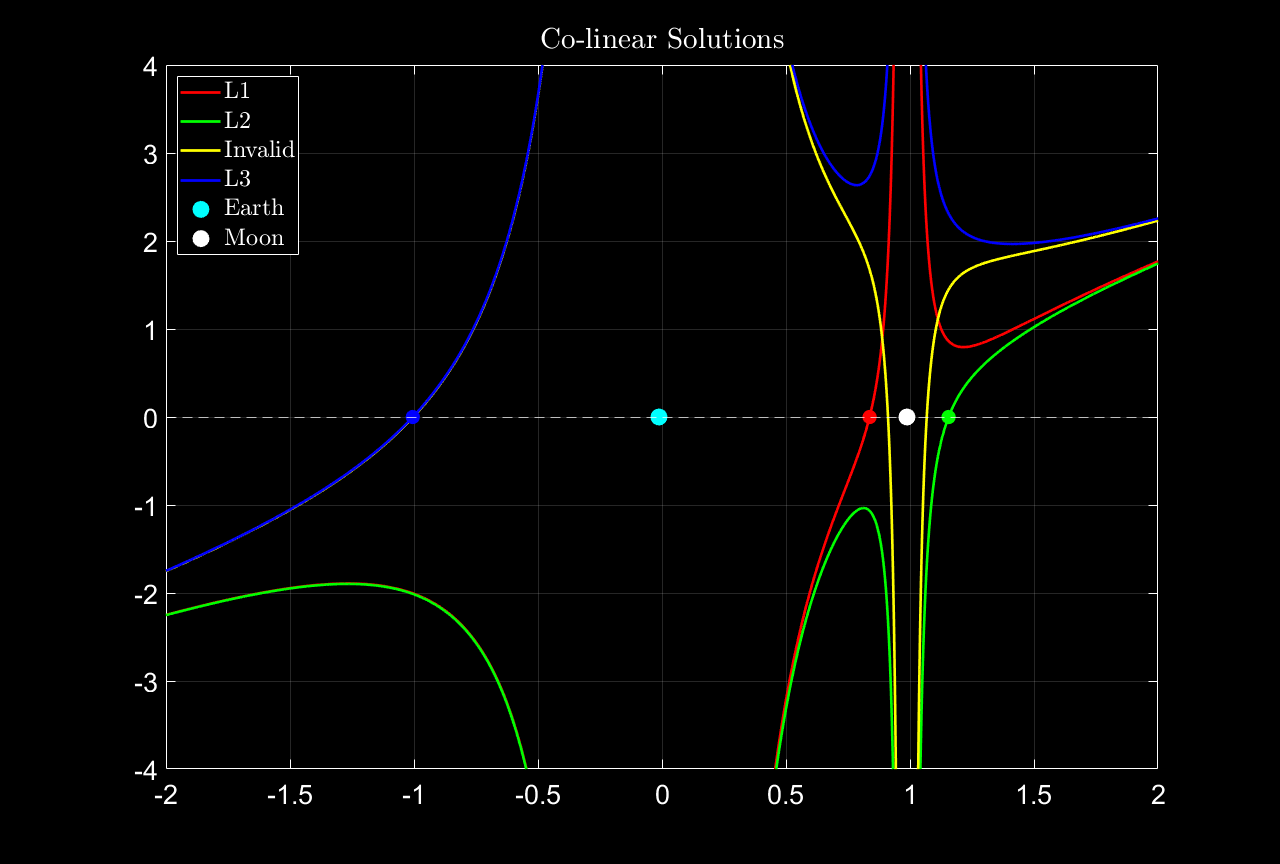
\includegraphics[width=\textwidth]{fig/lagrange123.png}
    \caption{Graphical Representation of the Collinear Solutions for the Lagrange points}
    \label{fig:lagrange_points}
\end{figure}

It is noted that these collinear solutions are determined using a numerical root-solving method (secant method) that utilizes finite differences for the estimation of derivatives and iteratively converges on the solutions. These solutions correspond to the x-coordinates of the Lagrange points ($L_1$--$L_3$), and the Earth and Moon are marked to indicate their relative positions in this configuration.

\vspace{\baselineskip}

\pagebreak

The coordinates of $L_1$, $L_2$, and $L_3$ are summarized below:

\begin{table}[h]
    \centering
    \caption{\cw Collinear Lagrange Points for Earth-Moon System}
    \begin{tabular}{ccc} \toprule
        {Lagrange Point} & {$x$} & {$y$}   \\ \midrule
        $L_1$ \cw  &  0.837023544523  & 0   \\
        $L_2$ \cw  &  1.155597402589  & 0   \\
        $L_3$ \cw  & -1.005053470159  & 0   \\  \bottomrule
    \end{tabular}
    \label{tab:table3}
\end{table}
\subsection*{\underline{Non-collinear Solutions (y $\neq$ 0)}:}

Let's bring back Equations~\eqref{eq:rootsY} \& \eqref{eq:rootsX}:
\begin{align*}
    \cm x \cw - \ddfrac{\left(1 - \cred \mu \cw \right) \left(\cm x \cw + \cred \mu \cw\right)}{\cc r_1 \cw ^3} - \ddfrac{\cred \mu \cw \left(\cm x \cw - 1 + \cred\mu\cw\right)}{\cg r_2 \cw ^3} &= 0
    \\
    \textcolor{magenta}{y} \left( 1 - \ddfrac{\left(1-\cred\mu\cw\right)}{\cc r_1 \cw ^3} - \ddfrac{\cred\mu\cw}{\cg r_2 \cw ^3} \right) &= 0
\end{align*}


Recalling the process for the collinear solutions, we looked at the trivial case where the variable $y$ is zero. The next step is to consider what occurs when $y$ is not assumed to be zero, which leads to setting the expression inside the parentheses of Equation~\eqref{eq:rootsY} to zero:

\begin{equation*}
    1 - \ddfrac{\left(1-\cred\mu\cw\right)}{\cc r_1 \cw ^3} - \ddfrac{\cred\mu\cw}{\cg r_2 \cw ^3} = 0 \\
\end{equation*}

However, this introduces a multivariable problem because the norms of the position vectors depend on both $x$ and $y$. Consequently, there are now two unknowns, $x$ and $y$, and two equations. To find a solution, the system of equations can be transformed into a linear system by implementing variable substitutions. This is done by defining new variables, $\alpha$ and $\beta$, to represent the reciprocal of the cube of the norm of the position vectors:

\begin{equation*}
    \cc \alpha \cw = \ddfrac{1}{\cc r_1 \cw ^3}, \quad \cg \beta \cw = \ddfrac{1}{\cg r_2 \cw ^3}
\end{equation*}

Subsituting these new variables into our system of non-linear equations:
\begin{align*}
    \cm x \cw - \left(1 - \cred \mu \cw \right) \left(\cm x \cw + \cred \mu \cw\right) \cc \alpha \cw 
    - \cred \mu \cw \left(\cm x \cw - 1 + \cred\mu\cw\right) \cg \beta \cw &= 0
    \\
    1 - \left(1-\cred\mu\cw\right) \cc \alpha \cw - \cred\mu\cw \cg \beta \cw &= 0
\end{align*}

Here, $\alpha$ \& $\beta$ are the independent variables we are solving for. Let's package these two equations into Matrix-vector form $[A]\underbar{\it{x}} + \underbar{\it{b}} = \underbar{0}$:

\begin{equation*}
    \begin{bmatrix}
        -\left(1 - \cred \mu \cw \right) \left(\cm x \cw + \cred \mu \cw\right)  &
        - \cred \mu \cw \left(\cm x \cw - 1 + \cred\mu\cw\right)
        \\
        - \left(1-\cred\mu\cw\right) &
        - \cred\mu\cw
    \end{bmatrix}
    \begin{bmatrix}
        \cc \alpha \\ \cg \beta
    \end{bmatrix}
    +
    \begin{bmatrix}
        \cm x \cw \\ 1
    \end{bmatrix}
    =
    \begin{bmatrix}
        0 \\ 0
    \end{bmatrix}
\end{equation*}

Inverting the system to solve for $\alpha$ \& $\beta$:

\begin{equation*}
    \begin{bmatrix}
        \cc \alpha \\ \cg \beta
    \end{bmatrix}
    = -
    \begin{bmatrix}
        -\left(1 - \cred \mu \cw \right) \left(\cm x \cw + \cred \mu \cw\right)  &
        - \cred \mu \cw \left(\cm x \cw - 1 + \cred\mu\cw\right)
        \\
        \cred\mu\cw - 1 &
        - \cred\mu\cw
    \end{bmatrix}^{-1}
    \begin{bmatrix}
        \cm x \cw \\ 1
    \end{bmatrix}
\end{equation*}

\end{document}